\section{Computing time bounds}

In this chapter we will present the method, which is able to infer time bounds for transitions of a program.
The original KoAT paper \cite{koat} presented two approaches: One basic approach, considering all transitions and a modular approach, considering a selected subset of transitions.
This master's thesis only considers the modular approach, since the other approach can just be defined as a special case of the modular approach, where the subset of transitions is the set of non-initial transitions $\TSet \setminus \TSet_0$.
The basis of the method are polynomial ranking functions.
The original KoAT allows the usage of arbitrary polynomial ranking functions.
But to obtain monotonicity, it uses an operator which considers the absolute values of variables and converts all negative signs in positive signs.
This is necessary to ensure, that a substitution of the variables with upper size bounds is still a sound overapproximation.
The new method only considers affine ranking functions, but does not need to apply such an operator.
Instead, the signs of the coefficients are considered and the appropiate upper or lower size bound is chosen respectively.
Note that the restriction to affine ranking functions is in practice not a major restriction, since most existing techniques also only generate affine ranking functions (e.g. \cite{podelski2004prf}, \cite{bradley2005linear}, \cite{bagnara2012new}, \cite{leike2014ranking}, \cite{ben2013linear}).

For the definition of the method we need to define the terms of entry locations and entry transitions.
We define the entry locations of a transition set $\TSet' \subseteq \TSet$ as $\mathcal{E}_{\TSet'} = \braced{\location_{in} \mid \TSet_{\location_{in}} \neq \emptyset \wedge \exists \location': (\location_{in}, \update, \guard, \location') \in \TSet'}$.
The entry transitions of a location $\location \in \mathcal{E}_{\TSet'}$ are defined as $\TSet_{\location} = \braced{(\location', \update, \guard, \location) \mid \exists \location', \update, \guard: (\location', \update, \guard, \location) \in \TSet \setminus \TSet'}$.
This is the same definition as used by the original KoAT \cite{koat}.

As an example, consider the program in figure \ref{fig:entrytransitions}.
The highlighted set of transitions $\TSet' = \braced{t_1, t_3, t_4}$ does have to entry locations $\mathcal{E}_{\TSet'} = \braced{\location_1, \location_2}$.
These entry locations define the entry transitions $\TSet_{\location_1} = \braced{t_0}$ and $\TSet_{\location_2} = \braced{t_2}$.

\begin{theorem}[TimeBounds]
  Let $(\UTime, \Size)$ be a complexity approximation. \\
  Let $\TSet' \subseteq \TSet \setminus \TSet_0$ a subset of all transitions such that $\TSet'$ contains no initial transitions. \\
  Let $\TSet_{\location} = \braced{(\location', \update, \guard, \location) \mid \exists \location', \update, \guard: (\location', \update, \guard, \location) \in \TSet \setminus \TSet'}$ denote the set of all transitions outside of the subprogram $\TSet'$ leading to an $\location \in \LSet$. \\
  Let $\mathcal{E}_{\TSet'} = \braced{\location_{in} \mid \TSet_{\location_{in}} \neq \emptyset \wedge \exists \location': (\location_{in}, \update, \guard, \location') \in \TSet'}$ denote the set of all entry locations of $\TSet'$. \\
  Let $\timerank: \LSet \rightarrow \BoundSet_a(\PVSet)$ be an \textbf{affine} time ranking function for $\TSet'$. \\
  For $t \in \TSet'_>$ let
  \[ \UTime'(t) = \sum_{\location \in \mathcal{E}_{\TSet'}} \sum_{\pret \in \TSet_\location} \UTime(\pret) \cdot \maxO{\usubst{\timerank(\location)}{\LSize(\pret)}{\USize(\pret)}} \]
  Let $\UTime'(t) = \UTime(t)$ for $t \in \TSet \setminus \TSet'_>$. \\
  Then, $\text{TimeBounds}(\UTime, (\USize, \LSize), \TSet') = \UTime'$ is also a runtime approximation.
\end{theorem}


\begin{figure}
  \centering
  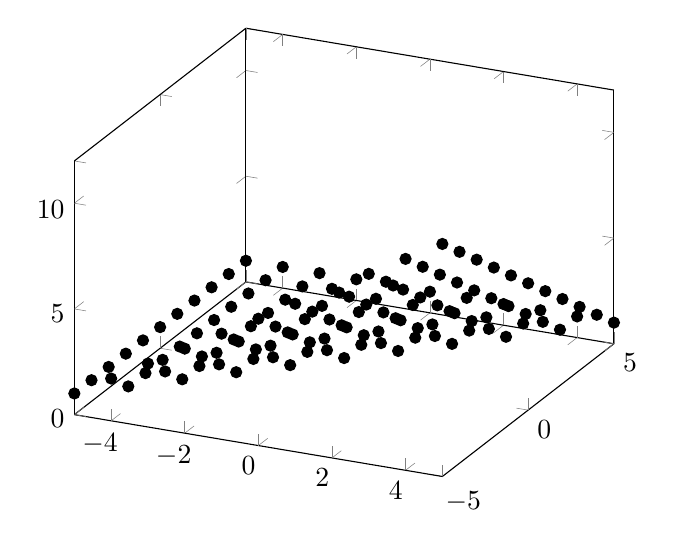
\begin{tikzpicture}
    \begin{axis}
      \addplot3 [
        unbounded coords=jump,
        mesh,
        shader=interp,
        samples at={-5,...,5},
        samples y={11},
        only marks,
      ] {1+max(x-y,0)};
    \end{axis}
  \end{tikzpicture}
  \hfil
  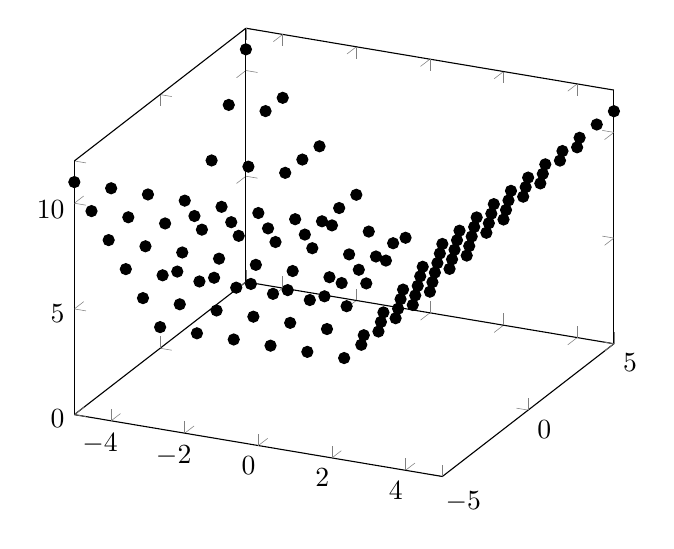
\begin{tikzpicture}
    \begin{axis}
      \addplot3 [
        unbounded coords=jump,
        mesh,
        shader=interp,
        samples at={-5,...,5},
        samples y={11},
        only marks,
      ] {1+abs(max(x,-y))+abs(max(x,-y))};
    \end{axis}
  \end{tikzpicture}
  \caption{Evaluation of the motivational example}
  \label{fig:motivational_evaluation}
\end{figure}


As an example, we consider the motivational program from the introduction \ref{fig:motivational_example}.
With the transition set $\TSet' = \braced{t_1}$ it is possible to determine a ranking function $\Pol(\location_1) = x - y$, since the transition $t_1$ decreases the measure and no transition increases the measure (since no other transition exists in $\TSet'$).
The old KoAT would now apply an operator to $\Pol$, such that the result would be a monotonic function with $\Pol'(\location_1) = \abs{x} + \abs{y}$.
The new method instead applies a split to $\Pol$, which results in the positive component $\Pol(\location_1)_+ = x$ and the negative component $\Pol(\location_1)_- = y$.
While the positive component $\Pol(\location_1)_+$ is a monotonically increasing function, the negative component $\Pol(\location_1)_-$ is a monotonically decreasing function.
Lets assume, that we already inferred the size bounds $\USize(t_0,x) = \LSize(t_0,x) = x$ and $\USize(t_0,y) = \LSize(t_0,y) = y$.
It is now possible to lift the components of the ranking functions to a global level with the substitution by the appropiate lower and upper size bounds $\eval{\Pol(\location_1)_+}{\USize(t_0)} - \eval{\Pol(\location_1)_-}{\LSize(t_0)} = x - y$.
Since with a state $\valuation$ with $\valuation(x) < \valuation(y)$ the transition $t_1$ will simply not occur in an evaluation instead of occuring a negative number of times, we have to ensure the positivity of $x - y$ with the operation $\maxO{x - y}$.
Then, the only step left is to consider the number of times an evaluation might enter the SCC from $t_0$.
Since $t_0$ is an initial transition, its time bound is $\UTime(t_0) = 1$.
Therefore an evaluation might only enter a single time from $t_0$ and the resulting time bound for $t_1$ is $\maxO{x - y}$.

\subsection{Choosing the transition set $\TSet'$}

\begin{figure}
\centering
\begin{tikzpicture}[->,>=stealth',auto,node distance=3cm,
    thick,
    main node/.style={circle,draw,font=\sffamily\Large\bfseries},
    aligned edge/.style={align=left}]

  \node[main node] (0) {$l_0$};
  \node[main node] (1) [right of=0] {$l_1$};
  \node[main node] (2) [right of=1] {$l_2$};
  \node[main node] (3) [right of=2] {$l_3$};

  \path[every node/.style={font=\sffamily\small}]
    (0) edge[aligned edge] node[above=0.2cm] {$t_0$} (1)
    (1) edge[aligned edge, loop above] node[above=0.2cm] {$t_1$} (1)
    (1) edge[aligned edge] node[above=0.2cm] {$t_2$} (2)
    (2) edge[aligned edge, bend left] node[above=0.2cm] {$t_3$} (3)
    (3) edge[aligned edge, bend left] node[below=0.2cm] {$t_4$} (2)
    ;
\end{tikzpicture}
\begin{tikzpicture}[->,>=stealth',auto,node distance=3cm,
    thick,
    main node/.style={circle,draw,font=\sffamily\Large\bfseries},
    aligned edge/.style={align=left}]

  \node[main node] (0) {$l_0$};
  \node[main node, dotted] (1) [right of=0] {$l_1$};
  \node[main node, dotted] (2) [right of=1] {$l_2$};
  \node[main node] (3) [right of=2] {$l_3$};

  \path[every node/.style={font=\sffamily\small}]
    (0) edge[aligned edge] node[above=0.2cm] {$t_0$} (1)
    (1) edge[aligned edge, ultra thick, loop above] node[above=0.2cm] {$t_1$} (1)
    (1) edge[aligned edge] node[above=0.2cm] {$t_2$} (2)
    (2) edge[aligned edge, ultra thick, bend left] node[above=0.2cm] {$t_3$} (3)
    (3) edge[aligned edge, ultra thick, bend left] node[below=0.2cm] {$t_4$} (2)
    ;
\end{tikzpicture}
\caption{A program for showing the difficulties of chosing the right subset of transitions}
\label{fig:entrytransitions}
\end{figure}


The choice of the transition set $\TSet'$ has a major impact on the quality of the time bounds.
Consider the program in figure \ref{fig:entrytransitions} with arbitrary guards and update for each transition.

A trivial approach would be to set $\TSet'$ to $\TSet \setminus \TSet_0 = \braced{t_1, t_2, t_3, t_4}$.
Then, we have $\mathcal{E}_{\TSet'} = \braced{\location_1}$ and $\TSet_{\location_1} = \braced{t_0}$.
Therefore for each $t \in \TSet'_>$ we end up with $\UTime'(t) = \UTime(t_0) \cdot \maxO{\eval{\Pol(\location_1)_+}{\USize(t_0)} - \eval{\Pol(\location_1)_-}{\LSize(t_0)}}$.
Since $t_0 \in \TSet_0$ is an initial transition, we have $\UTime(t_0) = 1$ and $\UTime'(t)$ then reflects the expected result of a non-modular approach.

This trivial approach requires us to find a ranking function, that satisfies the non-increasing constraint for all transitions.
If no such ranking function can be found, it is not possible to infer any time bounds with this transition set $\TSet'$.
But since the method allows us to only consider a subset of the transitions, it might be possible, to remove the transition which violates its non-increasing constraint.
Then, a ranking function could be found.

Let's assume that the transition violating the non-increasing constraint is $t_1$ and consider the transition set $\TSet' = \braced{t_3, t_4}$.
Since we reduced the set, we have fewer constraints and are more likely to find a ranking function.
We have $\mathcal{E}_{\TSet'} = \braced{\location_2}$ and $\TSet_{\location_2} = \braced{t_2}$.
Since $t_2$ is not part of a loop, its time bound is $\UTime(t_2) = 1$.
Therefore we end up with $\UTime'(t) = \maxO{\eval{\Pol(\location_2)_+}{\USize(t_2)} - \eval{\Pol(\location_2)_-}{\LSize(t_2)}}$.

Note that it is possible to select arbitrary subsets $\TSet' \subseteq \TSet$.
A non-connected subset $\TSet' = \braced{t_1, t_3, t_4}$ could be chosen, but would lead to a bound $\UTime'(t) = \maxO{\eval{\Pol(\location_1)_+}{\USize(t_0)} - \eval{\Pol(\location_1)_-}{\LSize(t_0)}} + \maxO{\eval{\Pol(\location_2)_+}{\USize(t_2)} - \eval{\Pol(\location_2)_-}{\LSize(t_2)}}$.
Also only a part of an SCC such as $\TSet' = \braced{t_4}$ could be chosen.
But since $t_3 \in \TSet_{\location_3}$ would be a entry transition of $\TSet' = \braced{t_4}$, this would only be of benefit if we already inferred a time bound $\UTime(t_3) < \infty$.

The implementation selects the transitions of the different SCCs of the program as transition set $\TSet'$ and excludes those transitions $t$, for which we already inferred a time bound $\UTime(t) < \infty$.
